\section{Lezione 20}

Per la documentazione si procede in modo \textbf{sequenziale} (vedere figura lezione precedente). La progettazione si fa andando ad esplodere le parti, dal grande al piccolo, in modo da agevolare i programmatori, i quali produrranno tanti moduli e li integreranno tra loro dopo la validazione. Noi vorremmo che dentro il repository ci vadano cose gi� buone, verificate in modo automatico e/o manuale (preferibilmente automatico, perch� la verifica manuale costa). La progettazione di dettaglio fissa unit�, fissa ci� che troveremo nel \textit{ramo ascendente} (vedi sempre figura). Quando ho unit� buone le posso mettere insieme (test di integrazione). Quando tutte le parti sono messe insieme allora posso fare un test di sistema. Nel percorso discendente il lavoro che riguarda la qualit� deve includere specifiche progressive delle verifiche che far� per la produzione. Noi vorremmo individuare un problema in modo facile, se � presente. Stadi di preparazione dei documenti:

\begin{center}
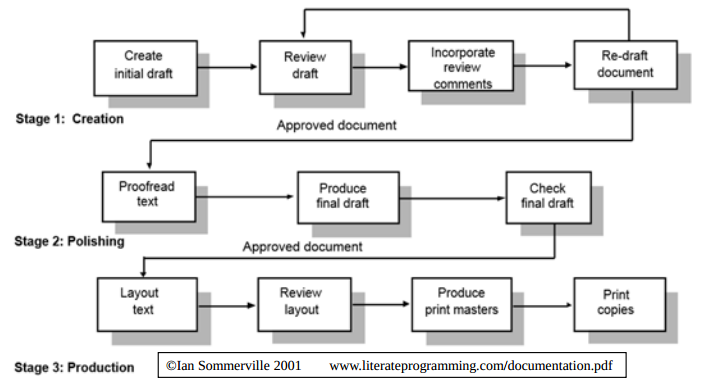
\includegraphics[width=0.75\columnwidth]{img1} % Example image
\end{center}

Tre momenti nella produzione dei documenti:

\begin{itemize}

	\item \textbf{Creazione};
	\item \textbf{Pulitura};
	\item \textbf{Rilascio}.

\end{itemize}

Le transizioni tra uno stato e l'altro hanno l'etichetta di ``\textit{documento approvato}''. Tutto ci� che facciamo in discesa implica ci� che faremo in salita, e tutto ci� che facciamo in salita motiva quello che sta in discesa. Il \textbf{tracciamento dei requisiti} pu� essere fatto:

\begin{itemize}

	\item \textbf{In avanti}: ``non mi dimentico niente'', devo portare tutto avanti in ogni passo;
	\item \textbf{All'indietro}: ogni modulo � necessario che sia l�.

\end{itemize}

Il tracciamento dev'essere assicurato ed automatizzato il pi� possibile. Dobbiamo avere \textbf{evidenza di copertura}. � un lavoro potenzialmente oneroso e non pu� essere fatto a mano. I requisiti andranno identificati attraverso codici che li renderanno \textbf{univoci}. Un codice che definisca di cosa stiamo parlando (es. RU). Poi dovr� numerarli in modo gerarchico, in cui c'� uno spazio e un ambito. Non un numero in modo sequenziale ma raggruppato attorno a \textbf{categorie}. Non devo avere necessariamente solo numeri ma posso avere anche lettere.

\textbf{Matrice di tracciamento}. Un requisito � buono se � facilmente verificabile. Ho bisogno di dare una struttura che mi faccia capire presto quanto le cose mi costeranno. � molto importante avere un \textbf{manuale utente}, che dev'essere scritto in modo che l'utente capisca. Un manuale serve come informazione supplementare (meglio una clip video rappresentativa). Si usa uno stile molto succinto e sintetico, non narrativo, in forma attiva (``questo fa questo''). \textbf{Tipi di manuali}:

\begin{center}
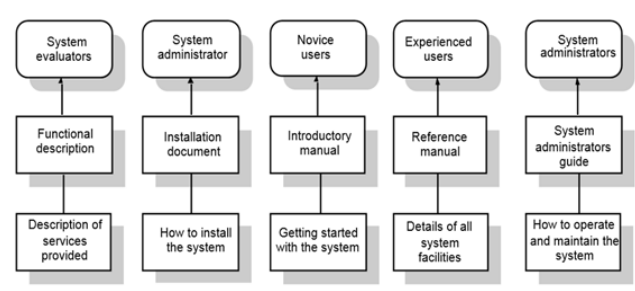
\includegraphics[width=0.75\columnwidth]{img2} % Example image
\end{center}

Stile di scrittura:

\begin{itemize}

	\item Forma attiva invece che passiva;
	\item Correttezza grammaticale e tipografica;
	\item Frasi brevi e intorno a un solo fatto;
	\item Usare liste piuttosto che frasi;
	\item Paragrafi brevi, fatti di poche frasi;
	\item Stile non verboso;
	\item Terminologia precisa (glossario);
	\item Usare pi� punti di vista per descrizioni complesse;
	\item Usare sezioni e sottosezioni titolate.

\end{itemize}

\textbf{Regole di progetto didattico}

C'� un rapporto strutturato fra i gruppi di progetto (fornitori) e il docente che rappresenta i proponenti (committente). Sar� un avanzamento regolato. Il cliente fissa un calendario e a una certa data vuole vedere determinate cose (Revisione di avanzamento). A questa revisione si accede facendo delle cose, operazioni obbligatorie e vincolanti. I documenti rappresentano l'oggetto di discussione sull'avanzamento.

\begin{center}
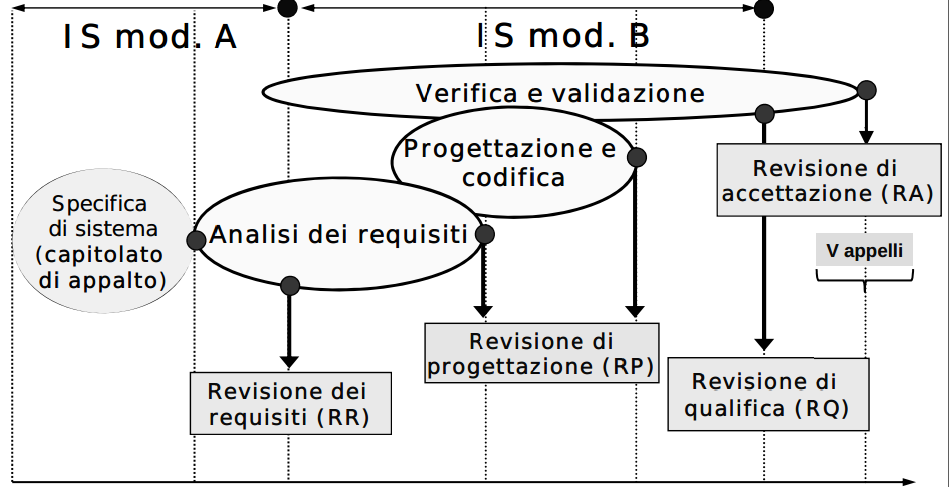
\includegraphics[width=0.75\columnwidth]{img3} % Example image
\end{center}

Per essere ammessi a diventare fornitori bisogna superare la revisione dei requisiti. Un po' di lavoro si sovrappone tra AR e progettazione. Le revisioni marcano uno stato di avanzamento. Il committente ad un certo punto vorr� vedere chi invitare al \textbf{collaudo}, chi avr� un software stabile. Il collaudo � posto temporalmente su uno dei 5 appelli del modulo B. La parte di tempo che sta nel modulo B finisce nella Revisione di Qualifica. Queste si chiamano \textbf{fasi esterne di progetto}, perch� per il committente sono viste come fasi di tempo contigue. In rapporto a SEMAT:

\begin{itemize}

	\item \textbf{Revisione dei requisiti};
	\item \textbf{Revisione di progettazione};
	\item \textbf{Revisione di qualifica};
	\item \textbf{Revisione di collaudo}.

\end{itemize}

Si esce dalla RR se i requisiti stanno tra \textbf{bounded} (perimetrati) e \textbf{acceptable} (negoziati). Arrivare ad avere la base di lavoro. Usciti da RP i requisiti sono tra acceptable e \textbf{addressed} e devo avere una buona architettura che soddisfi i requisiti (\textbf{architecture selected}. Uscito da RQ sono tra addressed e \textbf{fullfilled}, la progettazione e la codifica sono \textbf{usable}. Quando esco dalla RA ho i requisiti fullfilled e la progettazione � pronta (\textbf{ready}) per andare sul mercato.

Visione a calendario:

\begin{center}
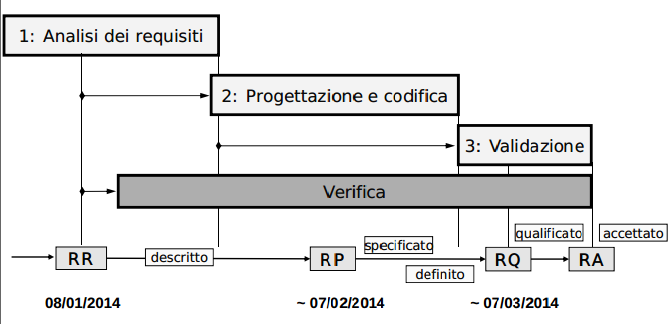
\includegraphics[width=0.75\columnwidth]{img4} % Example image
\end{center}

Temporalmente c'� almeno un mese tra una revisione e l'altra. Le revisioni hanno negli strati dell'ingegneria del software due possibili accezioni:

\begin{itemize}

	\item \textbf{Revisione formale}: c'� un arbitro esterno che d� un giudizio;
	\item \textbf{Revisioni di progresso}: sono delle discussioni paritarie, � come se ci fosse un consulente che valuta.

\end{itemize}

Le revisioni formali sono la prima (RR) e l'ultima (RA). Le altre sono di progresso, che servono per aiutare il gruppo a misurare il proprio avanzamento. Su ogni revisione ci sar� un voto (che fa media) e quelle formali sono \textbf{bloccanti}. Il voto di progetto conta per il 60\% del voto totale. Le revisioni si svolgono in ingresso con la presentazione di documentazione e poi con un colloquio orale e una discussione. Nelle revisioni interne ci sono degli obiettivi \textbf{tecnici} e \textbf{gestionali}. Per gestionali si intende l'avere una evidenza oggettiva che il progetto � sotto controllo per tempi, costi e avanzamento. Mostrare che l'avanzamento � coerente con le attese rispetto al modello di sviluppo utilizzato. Bisogna avere una \textbf{baseline}. Quando essa esiste allora siamo in grado di dimostrare che il progetto ha un progresso.

Nella Revisione dei Requisiti si entra con 3 documenti esterni e uno interno:

\begin{itemize}

	\item \textbf{Analisi dei requisiti}: spiega i requisiti derivati dal capitolato;
	\item \textbf{Piano di qualifica}: mette insieme verifica e validazione, che costituiscono la base della \textbf{qualit�}, ovvero tutto ci� che facciamo per ottenerla;
	\item \textbf{Piano di progetto}: la strategia per l'uso delle risorse intese come tempi, persone e gestione di queste due;

\end{itemize}

Il documento interno sono le \textbf{Norme di progetto}.

Nella Revisione di Progettazione devo avere due cose:

\begin{itemize}

	\item \textbf{Progettazione di alto livello};
	\item \textbf{Progettazione di dettaglio}.

\end{itemize}

Devo portare un documento che si chiama \textbf{specifica tecnica} e l'avanzamento incrementale di PQ e del PP in cui avremo un pezzo di consuntivo. Porto la \textbf{Definizione di prodotto}, dalla quale il programmatore inizier� il suo lavoro. Devo informare il cliente sulle caratteristiche del prodotto realizzato.

In RQ � finita la codifica oppure mancano pezzi non essenziali. Approvazione dell'esito finale della fase di verifica. Dovr� aggiornare la PQ e il PP e presentare una bozza del manuale utente.

Nella RA porto il prodotto finale \textbf{ultimato}. Adempimento del fornitore:

\begin{center}
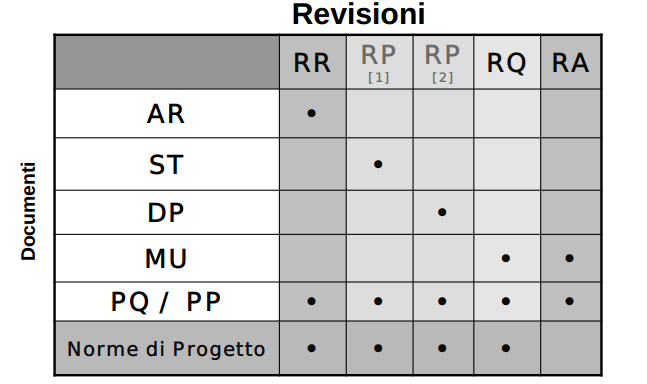
\includegraphics[width=0.75\columnwidth]{img5} % Example image
\end{center}